\documentclass{article}

\usepackage{fancyhdr}
\usepackage{lastpage}
\usepackage{extramarks}
\usepackage[usenames,dvipsnames]{color}
\usepackage{amsmath}
\usepackage{amsthm}
\usepackage{amsfonts}
\usepackage{changepage}
\usepackage{lineno}
\usepackage[plain]{algorithm}
\usepackage{algpseudocode}
\usepackage{hyperref}
\usepackage{tikz}

\topmargin=-0.45in
\evensidemargin=0in
\oddsidemargin=0in
\textwidth=6.5in
\textheight=9.0in
\headsep=0.25in

\linespread{1.1}

\pagestyle{fancy}
\lhead{\hmwkAuthorName}
\chead{\hmwkClass\ (\hmwkClassInstructor\ \hmwkClassTime): \hmwkTitle}
\rhead{\firstxmark}
\lfoot{\lastxmark}
\cfoot{}

\renewcommand\headrulewidth{0.4pt}
\renewcommand\footrulewidth{0.4pt}

\setlength{\floatsep}{100pt}
\renewcommand{\algorithmicrequire}{\textbf{Input:}}
\renewcommand{\algorithmicensure}{\textbf{Output:}}
\algrenewcomment[1]{\hfill // #1}

\setlength\parindent{0pt}

\hypersetup{colorlinks=true}

\newcommand{\enterProblemHeader}[1]{
    \nobreak\extramarks{}{Problem \arabic{#1} continued on next page\ldots}\nobreak{}
    \nobreak\extramarks{Problem \arabic{#1} (continued)}{Problem \arabic{#1} continued on next page\ldots}\nobreak{}
}

\newcommand{\exitProblemHeader}[1]{
    \nobreak\extramarks{Problem \arabic{#1} (continued)}{Problem \arabic{#1} continued on next page\ldots}\nobreak{}
    \stepcounter{#1}
    \nobreak\extramarks{Problem \arabic{#1}}{}\nobreak{}
}

\setcounter{secnumdepth}{0}
\newcounter{partCounter}
\newcounter{homeworkProblemCounter}
\setcounter{homeworkProblemCounter}{1}
\nobreak\extramarks{Problem \arabic{homeworkProblemCounter}}{}\nobreak{}

\newenvironment{homeworkProblem}{
    \section{Problem \arabic{homeworkProblemCounter}}
    \setcounter{partCounter}{1}
    \enterProblemHeader{homeworkProblemCounter}
}{
    \exitProblemHeader{homeworkProblemCounter}
}

\newcommand{\hmwkTitle}{Homework\ \#2}
\newcommand{\hmwkDueDate}{January 29, 2014}
\newcommand{\hmwkClass}{Stat330}
\newcommand{\hmwkClassTime}{Section A}
\newcommand{\hmwkClassInstructor}{Mr. Lanker}
\newcommand{\hmwkAuthorName}{Josh Davis}

\title{
    \vspace{2in}
    \textmd{\textbf{\hmwkClass:\ \hmwkTitle}}\\
    \normalsize\vspace{0.1in}\small{Due\ on\ \hmwkDueDate at 3:10pm}\\
    \vspace{0.1in}\large{\textit{\hmwkClassInstructor\ \hmwkClassTime}}
    \vspace{3in}
}

\author{\textbf{\hmwkAuthorName}}
\date{}

\newcommand{\alg}[1]{\textsc{\bfseries \footnotesize #1}}
\newcommand{\deriv}[1]{\frac{\mathrm{d}}{\mathrm{d}x} (#1)}
\newcommand{\dx}{\mathrm{d}x}
\newcommand{\solution}{\textbf{\large Solution}}

\renewcommand{\part}[1]{\textbf{\large Part \Alph{partCounter}}\stepcounter{partCounter}\\}


\begin{document}

\maketitle

\pagebreak


\begin{homeworkProblem}
    Binomial theorem.
    \\

    \part

    What is the coefficient of \(x^5 y^3\)?
    \\

    \solution

    \[
        c \cdot x^5 y^3 = \binom{8}{3} x^5 y^3= \frac{8!}{5!3!} x^5 y^3 = 56 x^5 y^3
    \]

    \part

    What is the coefficient of \(x^3 y^5\)?
    \\

    \solution

    \[
        c \cdot x^3 y^5 = \binom{8}{5} x^3 y^5= \frac{8!}{5!3!} x^3 y^5 = 56 x^3 y^5
    \]
\end{homeworkProblem}

\pagebreak

\begin{homeworkProblem}

\end{homeworkProblem}

\pagebreak

\begin{homeworkProblem}
    Let \(G\) and \(H\) be disjoint events in some sample space \(\Omega\).
    \\

    \part

    Describe the event \(G \cup H\).
    \\

    \solution

    A new event that includes outcomes in \(G\) \textbf{or} in \(H\).
    \\

    \part

    What is \(P(G \cup H)\) in terms of \(P(G)\) and \(P(H)\)?
    \\

    \solution

    Since \(G\) and \(H\) are disjoint, \(P(G \cap H) = 0\):

    \[
        \begin{split}
            P(G \cup H) &= P(G) + P(H) - P(G \cap H)
            \\
            &= P(G) + P(H) - 0
            \\
            &= P(G) + P(H)
        \end{split}
    \]
    \\

    \part

    Describe the event \(G \cap H\).
    \\

    \solution

    A new event that includes the outcomes that happen in event
    \(G\) \textbf{and} in \(H\).
    \\

    \part

    What is the probability of event \(G \cap H\)?
    \\

    \solution

    The probability of \(G \cap H = 0\) because the two events are disjoint.
\end{homeworkProblem}

\pagebreak

\begin{homeworkProblem}
    Venn diagrams. The grey areas indicate the solution.
    \\

    \part

    \(A \cup B\)
    \\

    \solution

    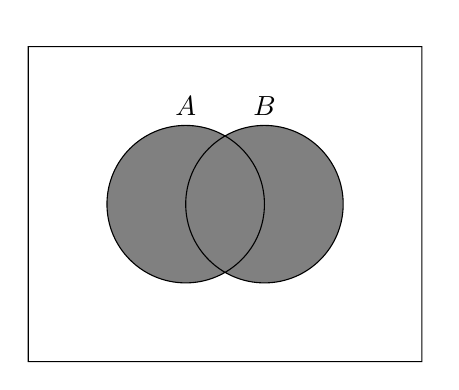
\begin{tikzpicture}[fill=gray]
        \begin{scope}
            \fill (0,0) circle (1);
            \fill (1,0) circle (1);
        \end{scope}

        \draw (0,0) circle (1) (0,1)  node [text=black,above] {$A$}
              (1,0) circle (1) (1,1)  node [text=black,above] {$B$}
              (-2,-2) rectangle (3,2) node [text=black,above] {};
    \end{tikzpicture}

    \part

    \(\overline{A \cup B}\)
    \\

    \solution

    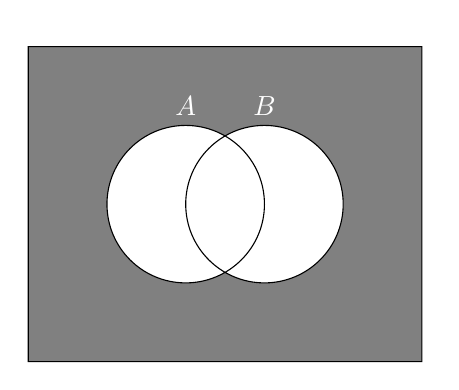
\begin{tikzpicture}[fill=gray]

        \begin{scope}
            \fill (-2,-2) rectangle (3,2);
        \end{scope}

        \begin{scope}
            \fill[white] (0,0) circle (1)
                         (1,0) circle (1);
        \end{scope}

        \draw (0,0) circle (1) (0,1)  node [text=white,above] {$A$}
              (1,0) circle (1) (1,1)  node [text=white,above] {$B$}
              (-2,-2) rectangle (3,2) node [text=black,above] {};
    \end{tikzpicture}

    \part

    \(\overline{A}\)
    \\

    \solution

    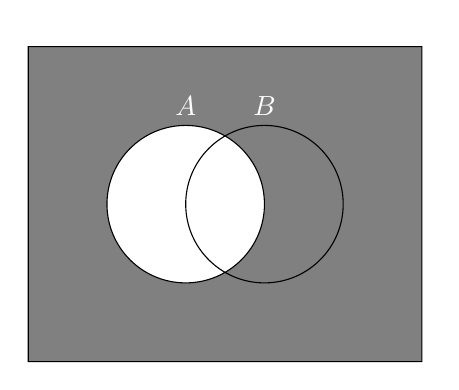
\begin{tikzpicture}[fill=gray]

        \begin{scope}
            \fill (-2,-2) rectangle (3,2);
        \end{scope}

        \begin{scope}
            \fill[white] (0,0) circle (1);
        \end{scope}

        \draw (0,0) circle (1) (0,1)  node [text=white,above] {$A$}
              (1,0) circle (1) (1,1)  node [text=white,above] {$B$}
              (-2,-2) rectangle (3,2) node [text=black,above] {};
    \end{tikzpicture}

    \pagebreak

    \part

    \(\overline{B}\)
    \\

    \solution

    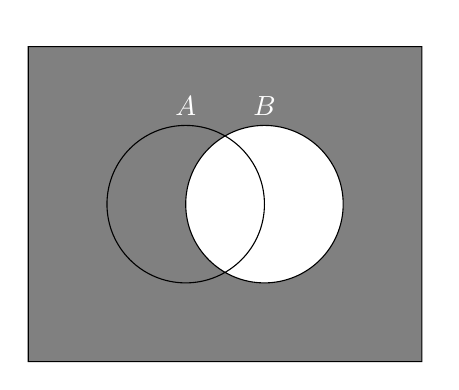
\begin{tikzpicture}[fill=gray]

        \begin{scope}
            \fill (-2,-2) rectangle (3,2);
        \end{scope}

        \begin{scope}
            \fill[white] (1,0) circle (1);
        \end{scope}

        \draw (0,0) circle (1) (0,1)  node [text=white,above] {$A$}
              (1,0) circle (1) (1,1)  node [text=white,above] {$B$}
              (-2,-2) rectangle (3,2) node [text=black,above] {};
    \end{tikzpicture}
    \\

    \part

    \(\overline{A} \cap \overline{B}\)
    \\

    \solution

    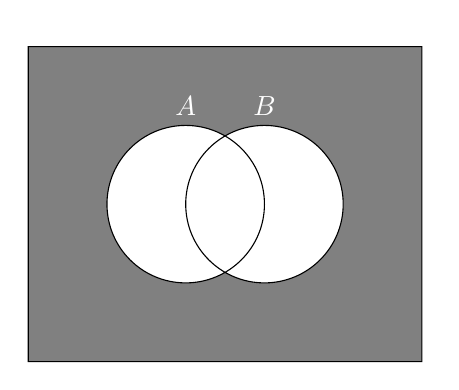
\begin{tikzpicture}[fill=gray]

        \begin{scope}
            \fill (-2,-2) rectangle (3,2);
        \end{scope}

        \begin{scope}
            \fill[white] (0,0) circle (1)
                         (1,0) circle (1);
        \end{scope}

        \draw (0,0) circle (1) (0,1)  node [text=white,above] {$A$}
              (1,0) circle (1) (1,1)  node [text=white,above] {$B$}
              (-2,-2) rectangle (3,2) node [text=black,above] {};
    \end{tikzpicture}

\end{homeworkProblem}

\pagebreak

\begin{homeworkProblem}
    Employees at a firm, 70\% know C, 60\% know Fortran and 50\% know both.
    \\

    \part

    Let \(A\) be the event that an employee knows C and \(B\) be the event that
    employee knows Fortran. Draw a Venn diagram.
    \\

    \solution

    \vspace{1in}

    \part

    What percentage of programmers do not know Fortran?
    \\

    \solution

    \[
        \begin{split}
            \Pr{(\neg \mbox{F})} &= 1 - \Pr{(\mbox{F})}
            \\
            &= 1 - .6
            \\
            &= .4
        \end{split}
    \]

    \part

    What percentage of programmers do not know Fortran and C?
    \\

    \solution

    \[
        \begin{split}
            \Pr{(\neg \mbox{F} \land \neg \mbox{C})} &= 1 - \Pr(\mbox{F} \lor \mbox{C})
            \\
            &= 1 - (\Pr(\mbox{F}) + \Pr(\mbox{C}) - \Pr(\mbox{F} \cap \mbox{C}))
            \\
            &= 1 - (.6 + .7 - .5)
            \\
            &= .2
        \end{split}
    \]

    \part

    What percentage of programmers know Fortran but not C?
    \\

    \solution

    \[
        \begin{split}
            \Pr{(\mbox{F} \land \neg \mbox{C})} &= \Pr{(F)} - \Pr{(\mbox{both})}
            \\
            &= .6 - .5
            \\
            &= .1
        \end{split}
    \]
\end{homeworkProblem}

\pagebreak

\begin{homeworkProblem}
    Total 60 students attending University. 9 were living off campus, 36 were
    undergrads, 3 were undergrads living off campus.
    \\

    Let \(A\) be the event denoting undergraduates and \(B\) denote living off campus.
    \[
        \begin{split}
            A &= 36
            \\
            B &= 9
            \\
            \overline{A} &= 60 - 36 = 24
            \\
            \overline{B} &= 60 - 9 = 51
            \\
            A \cap B &= 3
        \end{split}
    \]

    \part

    Number of students who were undergrads living on campus.
    \\

    \solution

    \[
        \begin{split}
            A \cap \overline{B} &= A \setminus B
            \\
            &= 36 - 9 + 3
            \\
            &= 30
        \end{split}
    \]
    \\

    \part

    Number of students who were graduate students living on campus.
    \\

    \solution

    \[
        \begin{split}
            \overline{A} \cap \overline{B} &= \overline{A} \setminus B
            \\
            &= 24 - 9 + 3
            \\
            &= 18
        \end{split}
    \]
\end{homeworkProblem}

\end{document}
